\documentclass[a4paper, 14pt]{article}

%\hypersetup
%{   colorlinks,
%    pdftitle={2.1.6. Journal},
%    pdfauthor={Володин Максим},
%    allcolors=[RGB]{010 090 200}
%}

\usepackage[T2A]{fontenc}
\usepackage[utf8]{inputenc}
\usepackage[english, russian]{babel}
\usepackage[top = 2cm, bottom = 2cm, left = 2cm, right = 2cm]{geometry}
\usepackage{indentfirst}
\usepackage{xcolor}
\usepackage{hyperref}
\usepackage{graphicx}
\usepackage{gensymb}
\usepackage{pgfplots}
\usepackage{amsmath, amsfonts, amssymb, amsthm, mathtools}
\usepackage{physics, multirow, float}
\usepackage{wrapfig, tabularx}
\usepackage{icomma} % Clever comma: 0,2 - number while 0, 2 - two numbers
\usepackage{tikz, standalone}
\usepackage{fancyhdr,fancybox}
\usepackage{lastpage}
\usepackage{booktabs}
\usepackage{listings}
\usepackage{lstmisc}

\graphicspath{{images/}}
\DeclareGraphicsExtensions{.pdf,.png,.jpg}

\restylefloat{table}
\usetikzlibrary{external}

\mathtoolsset{showonlyrefs = true} % Numbers will appear only where \eqref{} in the text LINKED
\pagestyle{fancy}

\pgfplotsset{compat=1.18}

\title {First document} %Заголовок, авторы, благодарности, дата
\author {Максим Володин}
% \thanks {funded by the Overleaf team}
\date {September 2022}

\begin{document} %Тело документа

    \maketitle
    We have now added a title, author and date to our first \LaTeX{} document!

    \tableofcontents

    \begin {abstract}
        This is a simple paragraph at the beginning of the document.
        A brief introduction about the main subject
    \end{abstract}

    Now that we have written our abstract, we can begin writing our first paragraph.

    This line will start a second Paragraph

    First document.
    This is a simple example, with no extra parameters pr packages included

    This universe is immense, and it seems to be homogeneous, in a large scale, everywhere we look at.

    \begin {figure} [h] %Вставка изображений
        \centering
        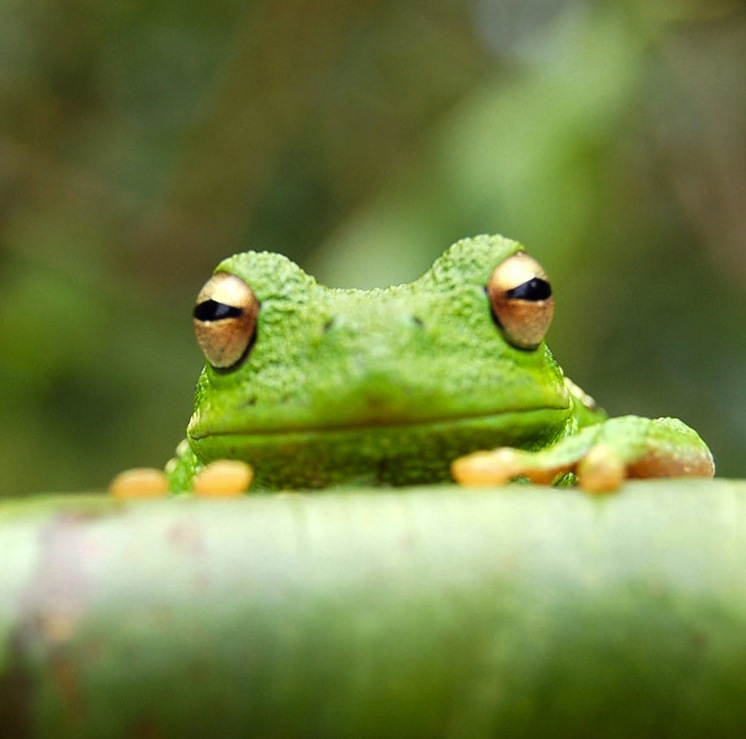
\includegraphics [width = 0.25\textwidth]{frog}
        \caption {a nice frog}
        \label{fig:mesh1}
    \end{figure}

    As you can see in the figure~\ref{fig:mesh1}, the function grows near 0.
    Also, in the page~\pageref{fig:mesh1} is the same example.

    There is a picture of a galaxy above

    %Игра с форматированием текста

    Some of the \textbf{greatest}
    discovers in \underline {science}
    were made by \textbf{\textit{accident}}.

    \texit {Some of the greatest \emph{discoveries} in science were made by accident.}

    %Маркированный список

    \begin {itemize}
        \item The individual entries are indicated with a black dot, a so-called bullet.
        \item The test in the entries may be of any length.
    \end {itemize}

    %Нумерованный список

    \begin{enumerate}
        \item This is the first entry in our list
        \item The list numbers increase with each entry we add
    \end{enumerate}

    In physics, the mass-energy equivalence is stated by the equation \[E=mc^2\] discovered in 1905 by Albert Einstein.
    In natural units ($c = 1$), the formula expresses the identity
    \begin{equation}
        E = m
    \end{equation}

    Subscripts in math mode are written as $a_b$ and superscripts are written as $a^b$.
    These can be combined as nested to write such s
    \[ T^{i_1 i_2 \dots i_p}_{j_1 j_2 \dots j_q} = T^(x^{i_1}, \dots, x^{i_p}, e_{j_1}, \dots, e_{j_q}) \]

    We write integrals using $\int$ and fractions using $\frac{a}{b}$.
    Limits are placed on integrals using superscripts and subscripts: \[\int_0^1 \frac{dx}{e^x} = \frac{e-1}{e} \]

    Lower case Greek letters are written as $\omega$ $\delta$ etc.
    while upper case Greek letters are written as $\Omega$ $\Delta$

    Mathematical operators are prefixed with a backslash as $\sin(\beta)$, $\cos(\alpha)$, $\log(x)$ etc.


    \chapter{First Chapter}


    \section{Introduction}

    This is the first section.

    Lorem ipsum dolor sit amet, consectetuer adipiscing elit.
    Etiam lobortisfacilisis sem.
    Nullam nec mi et neque pharetra sollicitudin.
    Praesent imperdietmi nec ante.
    Donec ullamcorper, felis non sodales\ldots


    \section{Second Section}

    Lorom ipsum dolor sit amet, consectetuer adispicing elit.
    Etiam lobortis facilisissem.
    Nullam nec mi et neque pharetra sollicitudin.
    Praesent imperdiet mi necante\ldots

    \subsection{First Subsection}
    Praesent imperdietmi nec ante.
    Donec ullamcorper, fellis non sodales\ldots

    \section*{Unnumbered Section} \addcontentsline{toc}{section}{Unnumbered Section}
    Lorem ipsum dolor sit amet, consectetuer adispicing elit.
    Etiam lobortis facilisissem

\end{document}